
\section{Introduction}

%\fixme{Decide the terminology: ReLU pruning or ReLU dropping}
% Privacy is important
Concerns surrounding data privacy continue to rise 
and are beginning to affect technology.
Companies are changing the way they use and store users' data
while lawmakers are passing legislation to improve users' privacy rights~\cite{hipaa, gdpr}.
Deep learning is the core driver of many applications impacted by privacy concerns.
It provides high utility in classifying, recommending, and interpreting user
data to build user experiences and requires large 
amounts of private user data to do so.
Private inference is a solution that simultaneously 
provides strong privacy guarantees while preserving the utility of neural networks 
to power application experiences users enjoy.
Today, in a typical inference pipeline, 
a client encrypts data (ciphertexts) and sends it to the cloud,
the cloud decrypts the data and performs inferences on the data (plaintext),
and returns the encrypted results.
With private inference, the same inference is executed
without the cloud ever decrypting the client's data;
that is, inferences are processed directly on ciphertexts.

\begin{figure}[t] \centering
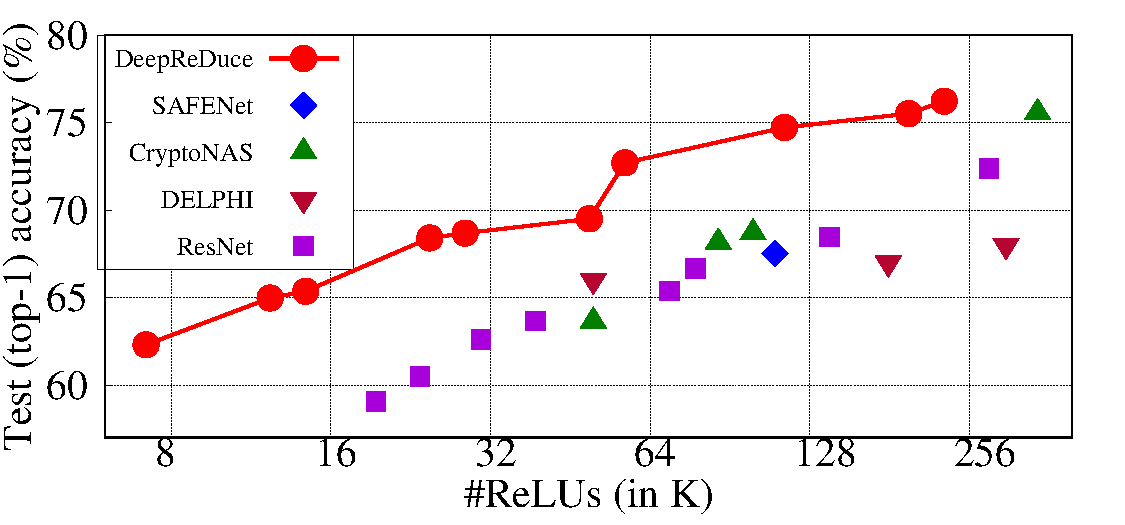
\includegraphics[scale=0.45]{Figures/ParetoFrontier}
\vspace{-2em}
\caption{DeepReDuce Pareto frontier of ReLU counts versus accuracy for CIFAR-100.
We show DeepReDuce outperforms
the state-of-the-art (SAFENet \cite{lou2021safenet}, CryptoNAS \cite{ghodsi2020cryptonas} and DELPHI \cite{mishra2020delphi}).}
%for private inference.}
\vspace{-2em}
\label{fig:ParetoFrontier}
\end{figure}

% Approaches and limitations
Prior work has established two methods for private inference.
The primary difference between them is how linear layers are computed,
either with secret-sharing (SS), a type of secure multi-party computation (MPC) \cite{goldreich2019play,shamir1979share}, or homomorphic encryption (HE), an encryption scheme that enables computation on ciphertexts \cite{gentry2009fully,brakerski2014efficient}.
For example, Gazelle~\cite{juvekar2018gazelle} and Cheetah~\cite{br2020cheetah} use HE for convolution and fully-connected layers
whereas MiniONN~\cite{liu2017oblivious}, DELPHI~\cite{mishra2020delphi}, and CryptoNAS~\cite{ghodsi2020cryptonas}
use SS. 
While distinct, both offer limited functional support and cannot readily process non-linear operations, e.g., ReLUs. 
To overcome this limitation, private inference protocols use Garbled circuits (GCs), another form of MPC \cite{yao1982protocols,yao1986generate}, to process ReLU privately.
%Switching between HE or SS to
However, GCs are several orders of magnitude more expensive than the linear layer protocols in terms of communication and computational, rendering private inference impractical~\cite{ghodsi2020cryptonas}.
For example, ReLUs account for 93\% of ResNet32's online private inference time using the DELPHI protocol~\cite{mishra2020delphi}.
Therefore, enabling low-latency private inference is a matter of minimizing a network's ReLU count. 

% Core contribution
%This paper investigates the relationship between the 
%ReLU count of a neural network and its overall accuracy.

To optimize networks for ReLU count we propose \emph{ReLU dropping}.
Inspired by weight and channel pruning methods that improve plaintext inference speed by reducing FLOPs, 
ReLU dropping directly reduces ReLU counts by removing entire ReLU layers from the network.
While weight and channel pruning also reduce ReLU counts, their ReLU savings are modest compared to FLOP savings.
%\footnote{For instance, scaling the number of channels in each layer by $\alpha$ reduces ReLU counts by $\alpha$ but FLOPs by $\alpha^{2}$.}.
In contrast, ReLU dropping achieves large reductions in ReLU counts by 
removing ReLU layers wholesale.
Leveraging our observations that
ReLU operators are unevenly distributed across network layers and
contribute differently to accuracy, we find ReLU dropping can be effectively 
applied to networks for large ReLU count reductions with minimal impact on accuracy.

%because even linear reductions in ReLU counts
%ReLU dropping selectively removes ReLUs operators to speedup private inference.
%While pruning methods also reduce ReLU counts, they only achieve modest reductions in 
%primary focus is on FLOPs; 
%cutting the number of channels in each layer by $2\times$ reduces ReLU count by $2\times$ but FLOPs by $4\times$
%Prior work has focused on replacing ReLUs with SS/HE amenable activations
%(e.g., X$^{2}$~\cite{gilad2016cryptonets,mishra2020delphi}) or proposed new network architectures that maximize weights per ReLU~\cite{ghodsi2020cryptonas}.
%This paper takes a novel and more direct approach by removing ReLUs wholesale.
%based on their 
%criticality, i.e., impact on the accuracy of network.
%ReLU dropping builds on our observations, described in Section~\ref{sec:Method}, that
%ReLU operators are unevenly distributed across network layers,
%contribute differently to accuracy,
%and that large fractions can be removed
%without significant accuracy loss.
%We show that 
%\fixme{SG: following sentence repetitive. remove?}
%Because ReLU operators dominate private inference run-time~\cite{ghodsi2020cryptonas},
%the optimizations result in significant latency improvement.


%We rigorously evaluate DeepReDuce using CIFAR-100, 
%the standard benchmark used for private inference~\cite{mishra2020delphi, ghodsi2020cryptonas}.
%Figure~\ref{fig:ParetoFrontier} shows that DeepReDuce's networks dominate 
%the ReLU count-accuracy Pareto frontier compared to CryptoNAS and DELPHI,  
%the current state of the art in private inference.


To further improve results we synergistically combine ReLU dropping with knowledge distillation (KD) \cite{hinton2015distilling,wang2021knowledge} to maximize the accuracy of optimized networks using the original Full-ReLU network.
We refer to our overall methodology as \emph{DeepReDuce}, 
which includes both optimizations for ReLU dropping and KD training.
%a method to optimize networks for private inference by selectively removing entire ReLU \fixme{layers}.
Figure~\ref{fig:ParetoFrontier} compares DeepReDuce against the current state-of-the-art: 
SAFENet \cite{lou2021safenet}, a method for selectively replacing channel-wise ReLUs with multiple degree and layer-wise mixed precision polynomials;
CryptoNAS~\cite{ghodsi2020cryptonas}, a neural architecture search (NAS) method targeting private inference and 
DELPHI~\cite{mishra2020delphi} a method for selectively substituting layer-wise ReLU activations with degree two polynomial activation functions.
We find that DeepReDuce significantly advances the accuracy-ReLU budget Pareto frontier across a wide design space.

% Discussion, answer obvious questions: Cant just train smaller network?
ReLU dropping has the added benefit that
when ReLUs are removed, the now adjacent linear transformations can be combined or merged, 
reducing the model depth and overall computations, i.e., FLOPs.
One obvious alternative to ReLU dropping is to simply start with shallower networks.
Our experiments show that DeepReDuce outperforms training shallower networks.
For example, ResNet9 (a down-scaled version of ResNet18, details in Section~\ref{sec:ExperimentalResults}) uses 30,720 ReLUs and and achieves 66.2\% accuracy 
whereas DeepReDuce produces a network with both \emph{fewer} ReLUs (24,600 ReLUs) and \emph{higher} accuracy (68.1\%).
%We note that the granularity of ReLU dropping is coarse.
%Therefore, we report numbers that show benefit in both ReLU count and accuracy.
We believe this is due to the fact that large models train better, 
which was also observed in \cite{zhao2018reThinking}. Detailed discussion is included in Section~\ref{subsec:ShallowResNet}.

% With respect to weight pruning, we first note that irregular weight pruning, such as~\cite{}, will not help as the distribution of remaining non-zero weights are random making it difficult to remove a significant number of ReLUs.
% Recent proposals for channel pruning~\cite{}, however, could help.
% In fact, one could interpret ReLU dropping as an extreme instance of channel pruning, 
% i.e., when all channels are pruned the effect is the same as removing a layer of ReLUs.
% However, channel pruning is not competitive with DeepReDuce and takes substantially longer to run.
% \fixme{We need data for this and to strengthen the text.
% Nandan, please enter your numbers.} \fixme{SG: agreed, this is critical imo b/c its the first in a reviewer would have.}

This paper makes the following contributions:
\begin{enumerate}
    \item Motivate the proposed idea of ReLU dropping and develop DeepReDuce:
            a method for the judicious removal of ReLUs to optimize networks
            for fast and accurate private inference.

    \item Rigorous evaluation of DeepReDuce demonstrating Pareto optimal designs across a wide range of       accuracy and ReLU counts. 
        DeepReDuce improves accuracy up to     
        3.5\% (iso-ReLU count) and reduces ReLUs by 3.5$\times$ (iso-accuracy) over the state of the art.

    %\item We conclude with a case study using TinyImageNet to demonstrate the generality of ReLU   
    %dropping beyond CIFAR-100 and ResNet.

    \item Show existing techniques for neural inference efficiency are insufficient for ReLU reduction and private inference. E.g., compared to the state-of-the-art channel pruning technique~\cite{he2020learning}, DeepReDuce provides a 2$\times$ greater ReLU reduction at with similar accuracy.
    %and provide a discussion of trade-offs in designing networks for small ReLU budgets.
    \end{enumerate}

%\fixme{Shall we add the performance comparison with SOTA pruning method here in contribution?}
